\documentclass[9pt,twocolumn,twoside,pdftex]{optica}

\usepackage{amsthm}
\newtheorem{definition}{Definition}
\newtheorem*{definition*}{Definition}


\setboolean{shortarticle}{false}
\setboolean{minireview}{false}



\title{Dual oxygen and temperature luminescence sensor based on artificial intelligence}

\author[1,2,*]{Francesca Venturini}
\author[2]{Umberto Michelucci}
\author[1]{Michael Baumgartner}

\affil[1]{Institute of Applied Mathematics and Physics, Zurich University of Applied Sciences,
Technikumstrasse 9, 8401 Winterthur, Switzerland}
\affil[2]{TOELT LLC; Birchlenstr. 25, 8600 Dübendorf, Switzerland}

\affil[*]{Corresponding author: francesca.venturini@zhaw.ch}


% To be edited by editor
% \dates{Compiled \today}

%\ociscodes{(300.6280) Spectroscopy, fluorescence and luminescence; (260.3800) Luminescence; (200.4260) Neural networks; (120.0280) Remote sensing and sensors.}

%https://www.osapublishing.org/submit/ocis/#230.0230
% To be edited by editor
% \doi{\url{http://dx.doi.org/10.1364/optica.XX.XXXXXX}}

\begin{abstract}
The optical determination of oxygen partial pressure is of great interest in numerous areas, like medicine, biotechnology, and chemistry. A well-known approach to the optical measure of oxygen is based on the quenching of luminescence by molecular oxygen . Sensors based on this principle typically rely on approximate empirical models to characterize the dependence of the luminescence intensity and decay time on the oxygen concentration through a multi-parametric model (Stern–Volmer equation), whose parameters are, however, all temperature-dependent. Therefore, the temperature needs to be known to determine the oxygen concentration and is measured separately, either optically or with a completely different sensor. In this work, we propose a new artificial intelligence  approach which allows the extraction of both the oxygen concentration and the temperature using one single indicator, which is sensitive to both oxygen and temperature, and measuring only the decay time. The results show that the neural network achieves predictions of both parameters which are comparable to the accuracy of commercial senors and therefore demonstrate the feasibility of this approach. Furthermore, the proposed artificial intelligence approach is not limited to oxygen and temperature sensing, but can be applied to luminescence of multiple indicators, whenever the underlying mathematical model is not known or too complex to derive the desired quantities from a single measurement.

\end{abstract}

\setboolean{displaycopyright}{true}

\begin{document}

\maketitle

\section{Introduction}

The simultaneous determination of multiple parameters can be very advantageous in many sensor applications, for example, when an in-situ or remote acquisition is required. If the measured parameters are interdependent or show cross-interference, their simultaneous determination becomes a necessity. Optical luminescence sensing is particularly attractive for multiple sensing. Using the same principle, several optical elements, like optical fiber and detector, can be shared in the setup for the detection of more than one parameter, thus allowing a compact and easy sensor design.

The typical approaches to multiple sensing are based on either the use of a single luminescence indicator (luminophore), whose luminescence is sensitive to more than one parameters or the use of several luminophores, one for each parameter, embedded in a substrate and placed in close physical proximity \cite{Stich2010,Borisov2011novel,Kameya2014,Wang2014,Santoro2016,Biring2019}. To be able to determine each parameter separately it is usually necessary to determine more than one optical property (e.g., absorption spectrum, emission spectrum, luminescence intensity, decay time) or to use special detection schemes to take advantage of the differences between optical properties of the used luminophores \cite{Collier2013,Wang2014,Stehning2004,Jorge2008,Biring2019,Moore2006}. 

The problem of dual sensing is particularly relevant in applications which involve oxygen sensing. The determination of oxygen partial pressure is of great interest in numerous fields, like medicine, biotechnology, environmental monitoring, or chemistry since oxygen plays an important role in many processes \cite{Papkovsky2013,Wang2014}. One of the most used optical measuring approaches uses the effect of the dynamical luminescence quenching by oxygen molecules. The measuring principle is based on the measurement of the luminescence of a specific luminophore, whose intensity and decay time are reduced due to collisions with molecular oxygen \cite{Lakowicz2006}.

Sensors based on this principle must rely on approximated empirical models to parametrize the dependence of the measured sensing quantity (e.g., luminescence intensity or decay time) on influencing factors of the environment where the indicator is placed. Among these, temperature is the parameter with the strongest influence since both the luminescence and the quenching phenomena are strongly temperature dependent. Therefore, in any optical oxygen sensor the temperature must be continuously monitored, most frequently with a separate sensor, and used to correct the calculated oxygen concentration \cite{Li2015}. This task can be difficult in a practical implementation and may be a major source of error in sensors based on luminescence sensing. Another disadvantage of this approach, is that the parametrization of the sensor response to temperature is system specific since it depends  on fabrication of the sensing element and of the sensor \cite{Xu1994,Draxler1995,Hartmann1996,Mills1998,Badocco2008,Dini2011}.

In this work we propose a revolutionary approach based on artificial intelligence which enables dual sensing, namely the determination of both the oxygen concentration and the temperature, using one single indicator and measuring a single quantity,  the decay time. Instead of describing the response of the sensor as a function of the relevant parameters through an analytical model, a neural network was developed and used to predict both oxygen concentration and temperature simultaneously.
For dual sensing, multi-task learning (MTL) neural networks are required, so networks which are characterized by common hidden layers, whose output is then the input of multiple branches of task specific hidden layers. This type of architectures, in facts, can learn correlated tasks \cite{Thrun1996, Caruana1997, Zhang2017, Baxter2000, Thung2018} and are flexible enough to be usable in multi-dimensional regressions \cite{Michelucci2019_2}.

The collection of the large amount of data which is needed for the training and test of neural networks, cannot be performed by hand. Therefore, a fully automated setup was developed which both controls the instruments for adjusting the sensing element environment, medium gas concentration and temperature, and collects the sensor response. This allowed the to collect enough measurements to train the neural network on real data and to test the sensor performance on other unseen real data.

This work proposes a paradigm shift from the classical description of the response of the sensor through an approximate empirical parametric model to the use of MTL neural networks. These which through the training on a large amount of data automatically taken will learn the complex inter-parameter dependencies and sensor-specific response characteristics, thus allowing enabling to build sensors even if the system is too complex, to be comfortably described by a mathematical model.



\section{Methods}
\label{sec:methods}

\subsection{Luminescence Quenching for Oxygen Determination}
\label{Theory}

Luminescence-based oxygen sensors usually consist of a dye molecule (luminophore) whose luminescence intensity and decay time decrease for increasing O$_2$ concentrations. This reduction is due to collisions of the excited luminophore with molecular oxygen, which thus provides a radiationless deactivation process (collisional quenching). 
In the case of homogeneous media characterized by an intensity decay which is a single exponential, the decrease in intensity and lifetime are both described by the Stern-Volmer (SV) equation \cite{Lakowicz2006}
\begin{equation}
\frac{I_0}{I}=\frac{\tau_0}{\tau}=1+K_{SV} \cdot \left[O_2\right]
\label{SVe}
\end{equation}
where $I_0$ and $I$, respectively, are the luminescence intensities in the absence and presence of oxygen, $\tau_0$ and $\tau$ the decay times in the absence and presence of oxygen, $K_{SV}$ the Stern–Volmer constant and $\left[O_2\right]$ indicates the oxygen concentration.

For practical applications, the luminophore needs to be embedded in a supporting substrate, frequently a polymer. As a result, the SV curve deviates from the linear behavior of equation (\ref{SVe}). This deviation can be due, for example, to heterogeneities of the micro-environment of the luminescent indicator, or to the presence of static quenching \cite{Wang2014}. A scenario which describes this non-linear behavior involves the presence in the substrate of two or more environments, in which the indicator is quenched at different rates \cite{Carraway1991,Demas1995}. This multi-site model describes the SV curve as the sum of two or more contributions as
\begin{equation}
\frac{I_0}{I}=\bigg[
\frac{f_i}{1+K_{SV,i} \cdot \left[O_2\right]}
\bigg]^{-1}
\label{SVe2}
\end{equation}
where $f_i$'s are the fractions of the total emission for each component under unquenched conditions, and $K_{SVi}$'s are the associated effective Stern–Volmer constants. Depending on the luminophore and on the substrate material, the models proposed in the literature may be even more complex \cite{Demas1995,Hartmann1995,Mills1999}.

In most industrial and commercial sensors, the decay time $\tau$ is frequently preferred to intensity measurement because of its higher reliability and robustness \cite{Wei2019}. The determination of the decay time is done most easily in the frequency domain by modulating the intensity of the excitation.  As a result, the emitted luminescence is also modulated but shows a phase shift $\theta$ due to the finite lifetime of the excited state. This method, has the advantage of allowing very simple and low-cost realization and is widely used in commercial applications.

Although the multi-site model was introduced for luminescence intensities, it is frequently also used to describe the oxygen dependence of the decay times \cite{Demas1995,Quaranta2012}. Therefore, in the simplest case of a two-sites scenario, the model can be rewritten in terms of phase shift as \cite{Michelucci2019}
\begin{equation}
\begin{aligned}
\frac{\tan \theta (\omega, T, [O_2])}{\tan \theta_0 (\omega, T)} =& \bigg( \frac{f (\omega , T) }{1+K_{SV1} (\omega , T) \cdot \left[O_2\right]}+ \\
&\frac{1-f (\omega , T) }{1+K_{SV2} (\omega , T) \cdot \left[O_2\right]} \bigg)^{-1} \\
\label{theta_full}
\end{aligned}
\end{equation}
where $\theta_0$ and $\theta$, respectively, are the phase shifts in the absence and presence of oxygen, $f$ and $1-f$ are the fractions of the total emission for each component under unquenched conditions, $K_{SV1}$ and $K_{SV2}$ are the associated Stern–Volmer constants for each component, and $\left[O_2\right]$ indicates the oxygen concentration. It is to be noted that the quantities $\theta_0$, $f$, $K_{SV1}$, and $K_{SV2}$ are all non-linearly temperature dependent \cite{Ogurtsov2006,lo2008,Zaitsev2016} and may result frequency dependent, an artifact of the approximation of the model. Finally, Eq. \ref{theta_full} needs to be inverted to determine $[O_2]$ from the measured quantity $\theta$.


\subsection{Experimental Setup}
\label{Experimental}

The optical setup used in this work for the luminescence measurements is shown schematically in Fig. \ref{fig:setup}. To be able to acquire a large number of data, both the software for the instrument control and for the data acquisition was written using the software LabVIEW by National Instruments. The acquisition procedure is described in detail in Sect. \ref{Data}.

\begin{figure}[htbp]
\centering
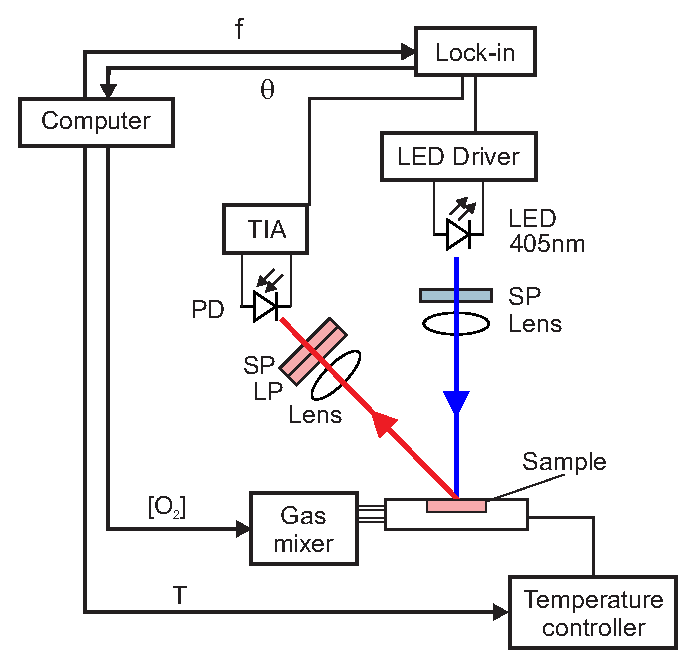
\includegraphics[keepaspectratio, width=8.4cm]{Setup_auto.eps}
\caption{Schematic diagram of the experimental setup. Blue indicates the excitation optical path, red the luminescence one. SP: short pass filter; LP: long pass filter PD: photodiode; TIA: trans-impedance amplifier.}
\label{fig:setup}
\end{figure}

The sample used for the characterization and test is a commercially available Pt-TFPP-based oxygen sensor spot (PSt3, PreSens Precision Sensing).
To control the temperature of the samples, these were placed in good thermal contact with a copper plate, placed in a thermally insulated chamber. The temperature of this plate was adjusted using a Peltier element and stabilized with a temperature controller (PTC10, Stanford Research Systems). The thermally insulated chamber was connected to a self-made gas-mixing apparatus which enabled to vary the oxygen concentration between 0 $\%$ and 20 $\%$ vol $O_2$ by mixing nitrogen and dry air from two bottles. In the following, the concentration of oxygen will be given in $\%$ of the oxygen concentration of dry air and indicated with $\%$ air. This means, for example, that 20 $\%$ air was obtained by mixing 20 $\%$ dry air with 80 $\%$ nitrogen and therefore corresponds to 4 $\%$ vol $O_2$. The absolute error on the oxygen concentration adjusted with the gas mixing device is estimated to be below 1 $\%$ air. 
 
The excitation light was provided by a 405 nm LED (VAOL-5EUV0T4, VCC Visual Communications Company LLC), filtered by a short pass (SP) filter with cut-off at 498 nm (Semrock 498 SP Bright Line HC short pass) and focused on the surface of the samples with a collimation lens. The luminescence was focused by a lens and collected by a photodiode (SFH 213 Osram).
To suppress stray light and light reflected by the sample surface, the emission channel was equipped with a long pass filter with cut-off at 594 nm (Semrock 594 LP Edge Basic long pass) and a short pass filter with cut-off at 682 nm (Semrock 682 SP Bright Line HC short pass). The driver for the LED and the trans-impedance amplifier (TIA) are self-made.
For the frequency generation and the phase detection a two-phase lock-in amplifier (SR830, Stanford Research Inc.) was used. 

\subsection{Automated Data Acquisition}
\label{Data}

The large amount of data needed for the training and the test of the neural network was acquired using an automated acquisition program which followed the flow-chart shown in Fig. \ref{fig:auto-data}. First, the program fixed the temperature and concentration. Then, the phase-shift was measured for varying modulation frequencies between 200 Hz and 15 kHz. This measurement was repeated 20 times. Next, keeping the temperature fixed, the program changed the oxygen concentration and the entire frequency-loop was repeated.
The oxygen concentration was varied between 0 $\%$ air and 100 $\%$ air in 5 $\%$ air steps.
Finally, the temperature was changed and then the oxygen and frequency loops where repeated. The temperature was varied between 5 $^\circ$C and 45 $^\circ$C in 5 $^\circ$C steps.
The total number of measurements was thus 50 x 20 x 21 x 9 = 189'000 which required a total acquisition time of approximately 65 hours. This number of measurement was chosen as a compromise between maximizing the number of data for the training of the neural network and avoiding photodegradation, which naturally occurs when the sample is subjected to illumination. A the end of the session a minimal change in the phase shift was observed.

\begin{figure}[t!]
\centering
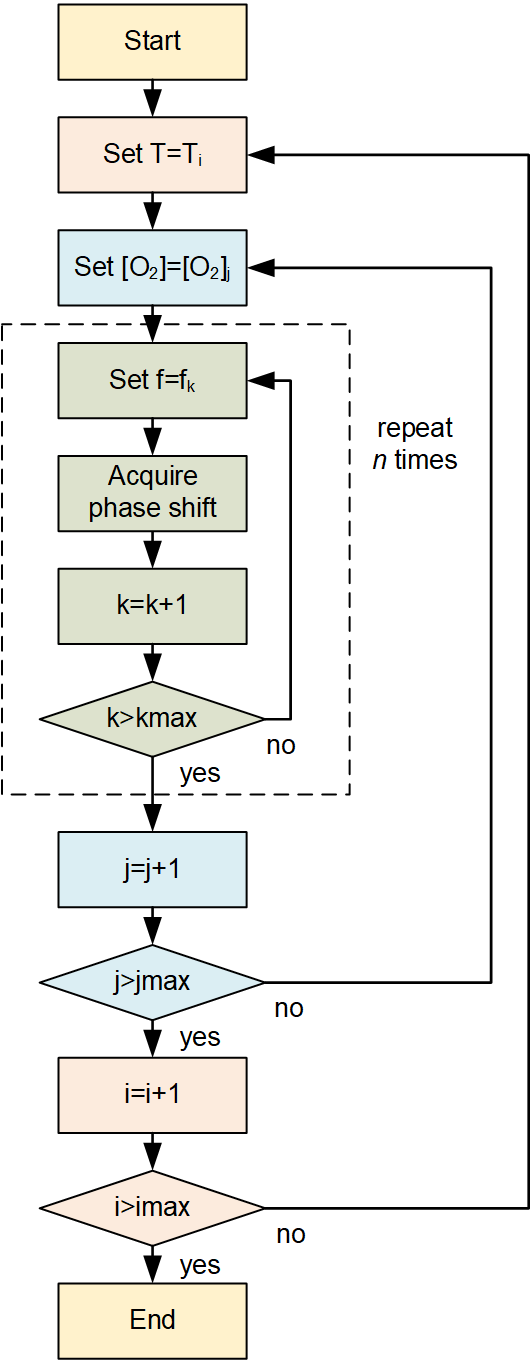
\includegraphics[keepaspectratio, width=5.9 cm]{flow-chart.png}
\caption{Flow-chart of the automatic measurement process.}
\label{fig:auto-data}
\end{figure}

%%%%%%% UMBI

\subsection{Neural Network Software}
\label{NN}



The software component of this new sensor type is based on a neural network model (NNM). A NNM is made of three components \cite{Michelucci2017}: a neural network architecture (that includes how neurons are connected, the activation functions and all the hyperparameters), a loss function (that we will indicate with $L$) and an optimiser algorithm. In this section those three components are described in detail.

\subsubsection{Neural Network Architecture}

The artificial network used in this work has a multi-task-learning architecture and is depicted in Figure \ref{fig:NN_MTL_O2_T}. It consists of three common hidden layers with 50 neurons each which generate as output a "shared representation". The name comes from the fact that the output of those layers is used to evaluate both $[O_2]$ and $T$. These are followed by three branches, two with each two additional "task-specific hidden layers" to predict respectively $[O_2]$ and $T$, and then one without additional layers to predict $[O_2]$ and $T$ at the same time.The shared representation is the input of two "task-specific hidden layers", that learn how to predict $[O_2]$ and $T$ better. This architecture uses the common hidden layers to find common features beneficial to each of the two tasks. During the training phase, learning to predict $[O_2]$ will influence the common hidden layers and therefore, the prediction of $T$, and vice-versa. The further task-specific hidden layers learn specific features to each output and therefore improve the prediction accuracy. The number of neurons of each task-specific hidden layer is 5. A study of which network architecture works best with this kind of data can be found in \cite{Michelucci2019}.

The sigmoid activation function was used as activation function for all the neurons. For all the runs presented in this article a starting learning rate of $\gamma = 10^{-3}$ has been used. Number of epochs and mini-batch size has been varied to optimize the NNM performance and are discussed in the appropriate sections. 

\subsubsection{Loss Function}

All the task specific loss functions $L_i$ used in this work are the mean square error (MSE), which is defined as
\begin{equation}
L_i = \frac{1}{n} \sum_{j=1}^n \sum_{k=1}^{d_i} (y_k^{[j]}-\hat y_k^{[j]})^2, \ \ \ i=1,2,3
\label{MSE}
\end{equation}
where $n$ is the number of observations in the input dataset; ${\mathbold y}^{[j]} \in \mathbb{R}^{d_i}$ is the measured value of the desired quantity for the $j^{th}$ observation (indicated as a superscript between square brackets), with $j=1, ..., n$ for the $i^{th}$ branch and $d_i$ is the dimension of the neural network branch output. In this case $d_1=2, d_2=1$ and $d_3=1$. $ \hat {\mathbold y}^{[j]} \in \mathbb{R}^{d_i}$ is the output of the network branch $i$, when evaluated on the $j^{th}$ observation. Since there are multiple branches, a global cost function $L$ needs to be defined as a linear combination of the task-specific cost functions with weights $\alpha_i$ 
\begin{equation}
L = \sum_{i=1}^{n_T}\alpha_i L_i .
\label{globalcf}
\end{equation}
The parameters $\alpha_i$ have to be determined during the hyper-parameter tuning phase to optimize the network predictions.
In this paper, being the cost function the MSE (Equation \ref{MSE}), the global cost function of Equation \ref{globalcf} is
\begin{equation}
L = \sum_{i=1}^{n_T}\alpha_i \frac{1}{n} \sum_{j=1}^n \sum_{k=1}^{d_i} (y_k^{[j]}-\hat y_k^{[j]})^2
\end{equation}
where  $n_T$ is the number of tasks; $n$ is the number of observations in the input dataset; ${\mathbold y}^{[j]} \in \mathbb{R}^d$ is the measured value of the desired quantity for observation $j$ from branch $i$, with $j=1, ..., n$; $ \hat {\mathbold y}^{[j]} \in \mathbb{R}^{d_i}$ is the output of the network, when evaluated on the $j^{th}$ observation.
The global cost function weights used for the plots were $\alpha_1 = 0.3$, $\alpha_2 = 5$ and $\alpha_3 = 1$. Those values were chosen because they result in the lowest $MAE$s (see discussion in Section \ref{Results} *****REFERENCE????*******).
 
\begin{figure}[htbp]
\centering
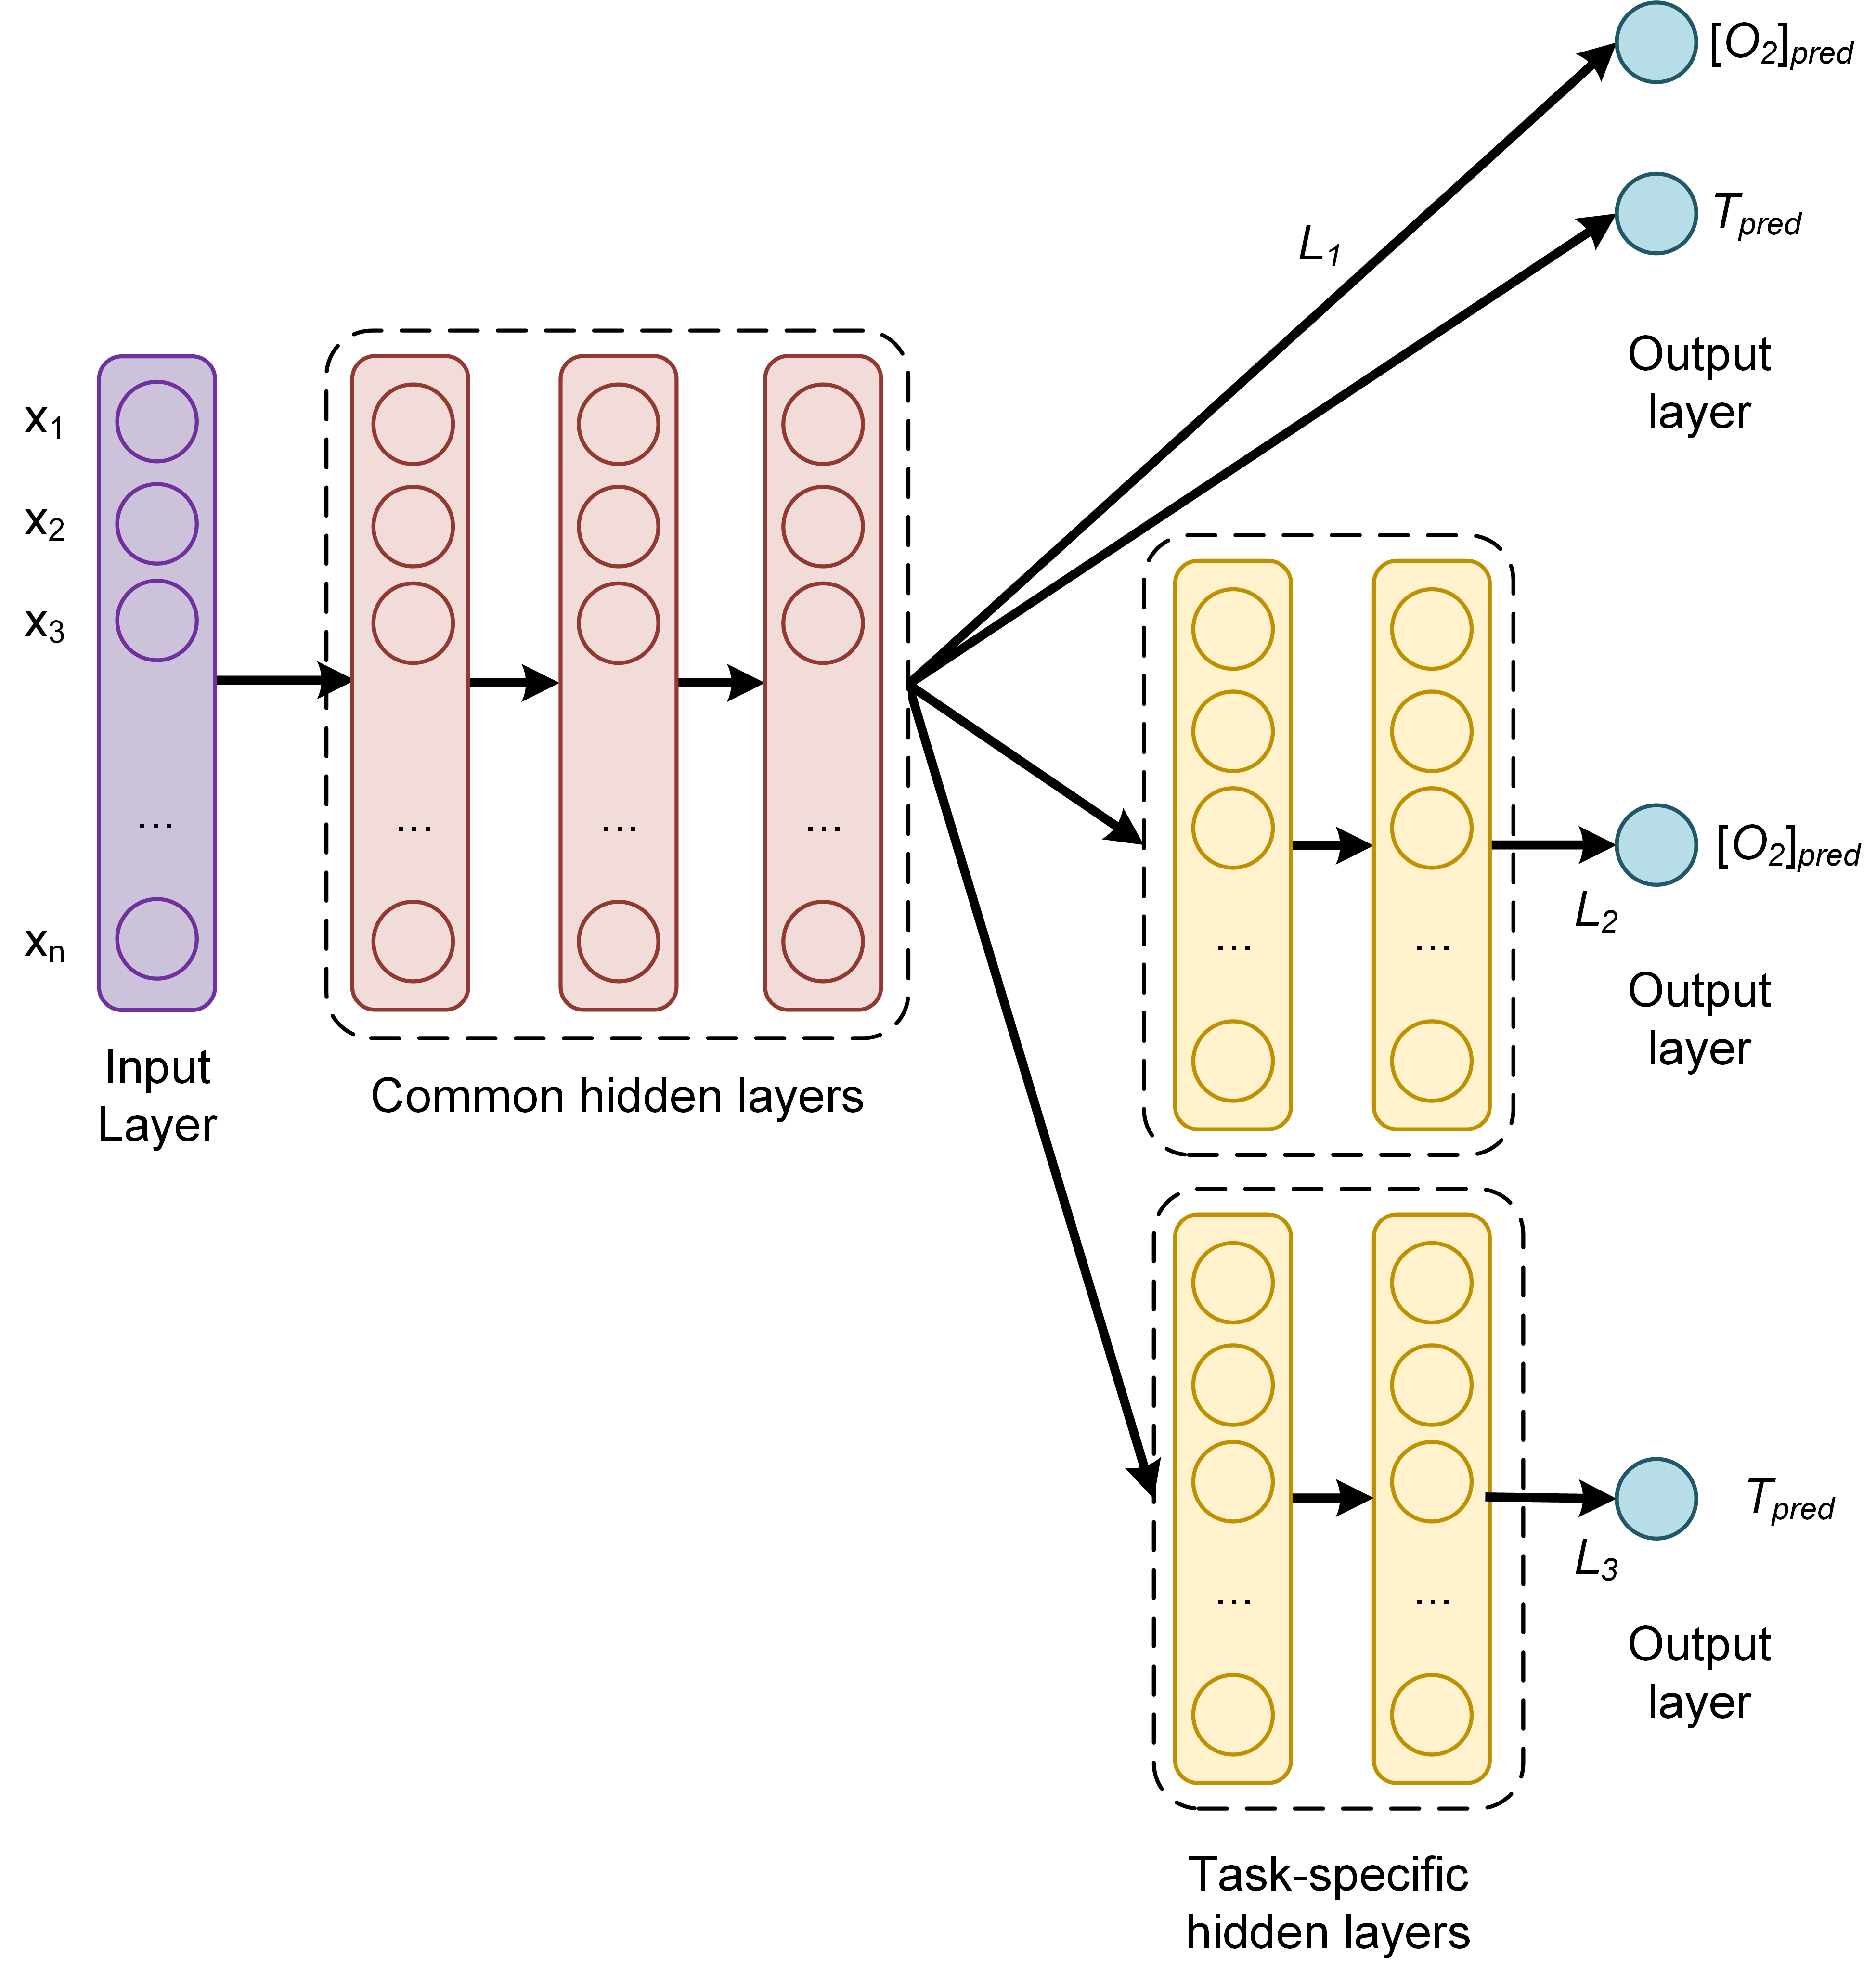
\includegraphics[width=8.7 cm]{NN_MTL_O2_T.png}
\caption{Architecture of the multi-task learning neural network used in this paper. The {\sl common hidden layers} generate as output a "shared representation" that is used as input to task specific branches that learn specific features to each quantity and therefore improve the prediction accuracy. } 
\label{fig:NN_MTL_O2_T}
\end{figure}


\subsubsection{Optimiser Algorithm}

To minimize the cost function, the optimizer Adaptive Moment Estimation (Adam) \cite{Kingma2014, Michelucci2017} was used. The training was performed with a starting learning rate of $10^{-3}$ as mentioned earlier. The neural network has been trained with two methods. 

{\bf No-batch training}:
with this method all the training data to evaluate the cost function is used to perform an update of the weights. The loss function used is the one in Equation (\ref{MSE}) where $n$ is the total number of observations available.

{\bf Mini-batch training}:
with this method a weight update is performed after the network has seen 32 observations. In this case the loss function is the one in Equation (\ref{MSE}) with $n=32$. For each weight update, 32 random observations are chosen from the training dataset without repetitions until all the training dataset has been fed to the network.  

No-batch training has the advantage of stabilty and speed, since it perform one weight update using the entire training dataset. Mini-batch training is normally much more effective, reaching lower values of the loss function in less epochs, but normally takes much more time \cite{Michelucci2017}. In our experiments No-batch training takes, for $20 \cdot 10^3$ epochs roughly 5 minutes on a modern macbook pro, while mini-batch training with $b=32$ takes, for the same amount of epochs, roughly 1 hour, so it is ca. 12 times slower, but is, as it will be shown later, much more effective in term of the neural network predictions. 
The implementation was performed using the TensorFlow\texttrademark $\ $library. 

\subsubsection{Predictions Absolute Error}

The metric used to compare predictions from expected values is the absolute error ($AE$) defined as the absolute value of the difference between the predicted and the expected value for a given observation. For the oxygen concentration predicted from branch $q$ for the 
$j^{th}$ observation $[O_2]^{[j]}$  the $AE$ is 
\begin{equation}
\label{AE}
AE^{q,{[j]}}_{[O_2]} = |[O_2]^{q,{[j]}}_{pred}-[O_2]^{[j]}_{meas}|.
\end{equation}
Note that in the architecture described in the previous sections, only branch 1 and 2 can predict $[O_2]$, while $T$ can be predicted by branch 1 and 3. In all the results shown in the following sections the predicted $[O_2]$ is from branch 2, while the predicted $T$ is from branch 3. The suffix $q$ in the predicted values will be therefore omitted.
The further quantity used to analyze the performance of the network is the mean absolute error ($MAE$), defined as the average of the absolute value of the difference between the predicted and the expected oxygen concentration or temperature. For example, for the oxygen prediction using the training dataset $S_{train}$, $MAE_{[O_2]}$ is defined as 
\begin{equation}
\label{MAE}
MAE_{[O_2]}(S_{train}) = \frac{1}{|S_{train}|} \sum_{j \in S_{train}}|[O_2]_{pred}^{[j]}-[O_2]_{real}^{[j]}|
\end{equation}
where $|S_{train}|$ is the size (or cardinality) of the training dataset. 
$AE_{T}$ and $MAE_T$ are similarly defined.


\subsubsection{Error Limited Accuracy $\eta$}
\label{sektion:ela}

To better characterise the sensor performance as a whole we need to define a new metric, that we have called Error Limited Accuracy (ELA), and that we indicate with $\eta$ that can be defined as follows.

\begin{definition*}
In a regression problem, given a metric $m$, and a certain value of it $\hat m$, the ELA for this metric $\eta$ limited by the error $\hat m$ is defined as the number of predictions $\hat y$ of the NNM that lie in the range $[m(\hat y)-\hat m, m(\hat y)+\hat m]$ divided by the total number of observations. It will be indicated with $\eta(\hat m)$. In more mathematical terms once we define the set
\begin{equation}
S(\hat m) = \{ \hat y^{[i]} \ {\text with } \ i = 1,..., n\ | |m(\hat y^{[i]})-m(y^{[i]})|\leq \hat m \} 
\end{equation}
$\eta$ can be simply defined as
\begin{equation}
\eta(\hat m) = \frac{|S(\hat m)|}{n}
\end{equation}
where $|S(\hat m)|$ is the cardinality of the set $S(\hat m)$ or in other words, the number of its elements.
\end{definition*}

This metric allows us to interpret the regression problem we are trying solve as a classification one. $\eta(\hat m)$ simply tells us how many observations are predicted by the NNM within a given value of the chosen metric $\hat m$. If we choose the metric $m$ as the $AE$ of the predictions, $\eta(AE)$ has a very intuitive and useful interpretation. 
In this case $\eta(\hat{m})$ with $\hat m = \hat{AE}$, is simply the percentage of predictions that are predicted within a certain error $\hat m$ from the expected values.
In this case, if we take $\hat m$ big enough, all the predictions will be classified perfectly. The smaller $\hat m$ the smaller the number of predictions correctly classified. 

\section{Results and Discussion}
\label{Results}

\subsection{Luminescence Experimental Results}

\begin{figure}[t!]
\centering

\includegraphics[width=8 cm]{phase_O2_T.eps}
\caption{Measured phase-shift as a function of the oxygen concentration, for selected temperatures at a fixed modulation frequency of 6 kHz. The arrow marks increasing temperatures.}
\label{fig:expdata1}
\end{figure}

As described in Section \ref{Theory}, the phase-shift depends not only on the oxygen concentration, but also on the temperature and on the modulation frequency of the excitation light. This can be seen in the Figs. \ref{fig:expdata1} to \ref{fig:expdata3}.
Fig. \ref{fig:expdata1} shows the measured phase shifts as a function of the oxygen concentration at a constant modulation frequency of 6 kHz for increasing temperatures. For clarity, only selected temperatures are shown. The decrease in the phase shift with increasing concentration is due to the quenching of the luminescence described in Eq. \ref{theta_full}. The effect of the temperature is to further decrease the phase shift. This effect depends on the concentration, being stronger at higher oxygen concentration. This temperature quenching is understandable since higher temperature increase diffusion of the oxygen molecules. {\bf [REF]}



For a given oxygen concentration the phase shift is strongly dependent from the modulation frequency, as it can be seen in Fig. \ref{fig:expdata2}. The temperature quenching is visible in the reduction of the phase shift with increasing temperatures at a given modulation frequency. This affects the phase shift differently depending on the modulation frequency. 

\begin{figure}[h!]
\centering

\includegraphics[width=8 cm]{phase_f_T.eps}
\caption{Measured phase-shift for selected oxygen concentrations as a function of the modulation frequency at a fixed oxygen concentration $[O_2]=20 \%$ at selected temperatures.}
\label{fig:expdata2}
\end{figure}

The complementary to Fig. Fig. \ref{fig:expdata2} is  Fig. \ref{fig:expdata3}, where the phase shift is shown a function of the modulation frequency for selected oxygen concentrations at a fixed temperature.

\begin{figure}[htbp]
\centering

\includegraphics[width=8 cm]{phase_f_O2.eps}
\caption{Measured phase-shift for selected oxygen concentrations as a function of the modulation frequency at a fixed temperature $T=25 ^{\circ}$ .}
\label{fig:expdata3}
\end{figure}

Comparing the curves shown above it is clear that, when measuring one single phase-shift or even a the phase-shift as a function of the modulation frequency is not possible to simultaneously determine both the oxygen concentration and the temperature from this set of data from Eq. (\ref{theta_full}). The temperature must be known to be able to determine the oxygen concentration. This is no longer the case with the artificial intelligence approach, as it will be shown in the next section. 

\subsection{Sensor performance analysis}

\subsubsection{Kernel Density Estimation}

To analyze the performance of the network, a fundamental quantity is the prediction probability density distribution of the $AE$s since it carries information on the probability of the network to predict the expected value for each parameter. For this reason and to make a clear visualisation of the results the  kernel density estimate (KDE) of the distributions of the $AE$s for both the oxygen concentration and the temperature was calculated. KDE is a non-parametric algorithm to estimate the probability density function of a random variable by inferring the population distribution based on a finite data sample \cite{Hastie2009}. 
In this work a Gaussian Kernel and a Scott bandwidth adaptive estimation \cite{Sain1996} using the seaborn Python package \cite{Waskom2020} were used.


\subsection{Sensor performance}

Let's start with discussing what is the effect of using mini-batches versus not using them. The results can be seen for  $AE_{[O_2]}$ and $AE_T$  in Figure \ref{fig:KDE_results_all}(A) and \ref{fig:KDE_results_all}(B) respectively. For this comparison the network has been trained for 20000 epochs. In the Figure the gray histogram shows the results when using mini-batches of size 32. The effect is extraordinary. The predictions move from (without using batches) having MAE$_{[O_2]}=2.38$ \% air and MAE$_{T}=3.63^\circ$ C to  
MAE$_{[O_2]}=1.36$ \% air and MAE$_{T}=1.63^\circ$ C (while using mini-batches of size 32). Not only the average values are reduced but the predictions distributions are much narrower. From Figure \ref{fig:KDE_results_all}(A) and \ref{fig:KDE_results_all}(B) it can also be clearly seen that, even while using mini-batches, we can get errors as high as roughly 5 \% air for $[O_2]$ or roughly as 12 $^\circ$ C for $T$. While deciding what is the right mini-batch size, training time must be taken into account. In fact decreasing the mini-batch size have the side effect of increasing the training time. While training the network without batches requires just a few minutes, reducing the mini-batch size to 32 increase the training time to roughly 1 hour.

\begin{figure*}[htbp]
\centering
\includegraphics[width=17 cm]{KDE_results_all.eps}
\caption{Performance of the neural network for the oxygen (left plot) and for the temperature (right plot) predictions: Normalized prediction distribution histogram (columns) and kernel density estimate (KDE) of the distribution of the $AE$s (solid line) using plain gradient descent (GD) and using mini-batches (MB) with a batch size of 32. The corresponding $MAE$ is also shown as a dashed line in each diagram.}
\label{fig:KDE_results_all}
\end{figure*}

%\begin{figure*}[htbp]
%\centering
%\includegraphics[width=17 cm]{prediction_distribution_batch.eps}
%\caption{Performance of the neural network for the oxygen (left plot) and for the temperature (right plot) predictions: Normalized prediction distribution histogram (columns) and kernel density estimate (KDE) of the distribution of the $AE$s (solid line) using plain gradient descent (GD) and using mini-batches (MB) with a batch size of 32. The corresponding $MAE$ is also shown as a dashed line in each diagram.}
%\label{fig:prediction_distribution_batch_90}
%\end{figure*}

One can get much better results simply training the network for many more epochs. In Figure \ref{fig:KDE_results_all}(C) and \ref{fig:KDE_results_all}(D) the difference between predictions distributions with 20000 and 100000 epochs (always using a mini-batch of size 32) is shown. The results are dramatically better. When the network has been trained for 100000 epochs we have a MAE$_{[O_2]}=0.22$ \% air and a MAE$_{T}=0.27^\circ$ C. Additionally all the predictions for $[O_2]$ lies below 0.94 \% air, and for $T$ lie below 2.1 $^\circ$ C. To train a network for so many epochs requires, on a modern laptop, roughly 5 hours. Predicting both $[O_2]$ and $T$ at the same time from the same set of data with such accuracies is unprecedented and paves the way to a completely new generation of sensors that does not need to measure temperature independently to predict the oxygen concentration.

%\begin{figure*}[htbp]
%\centering
%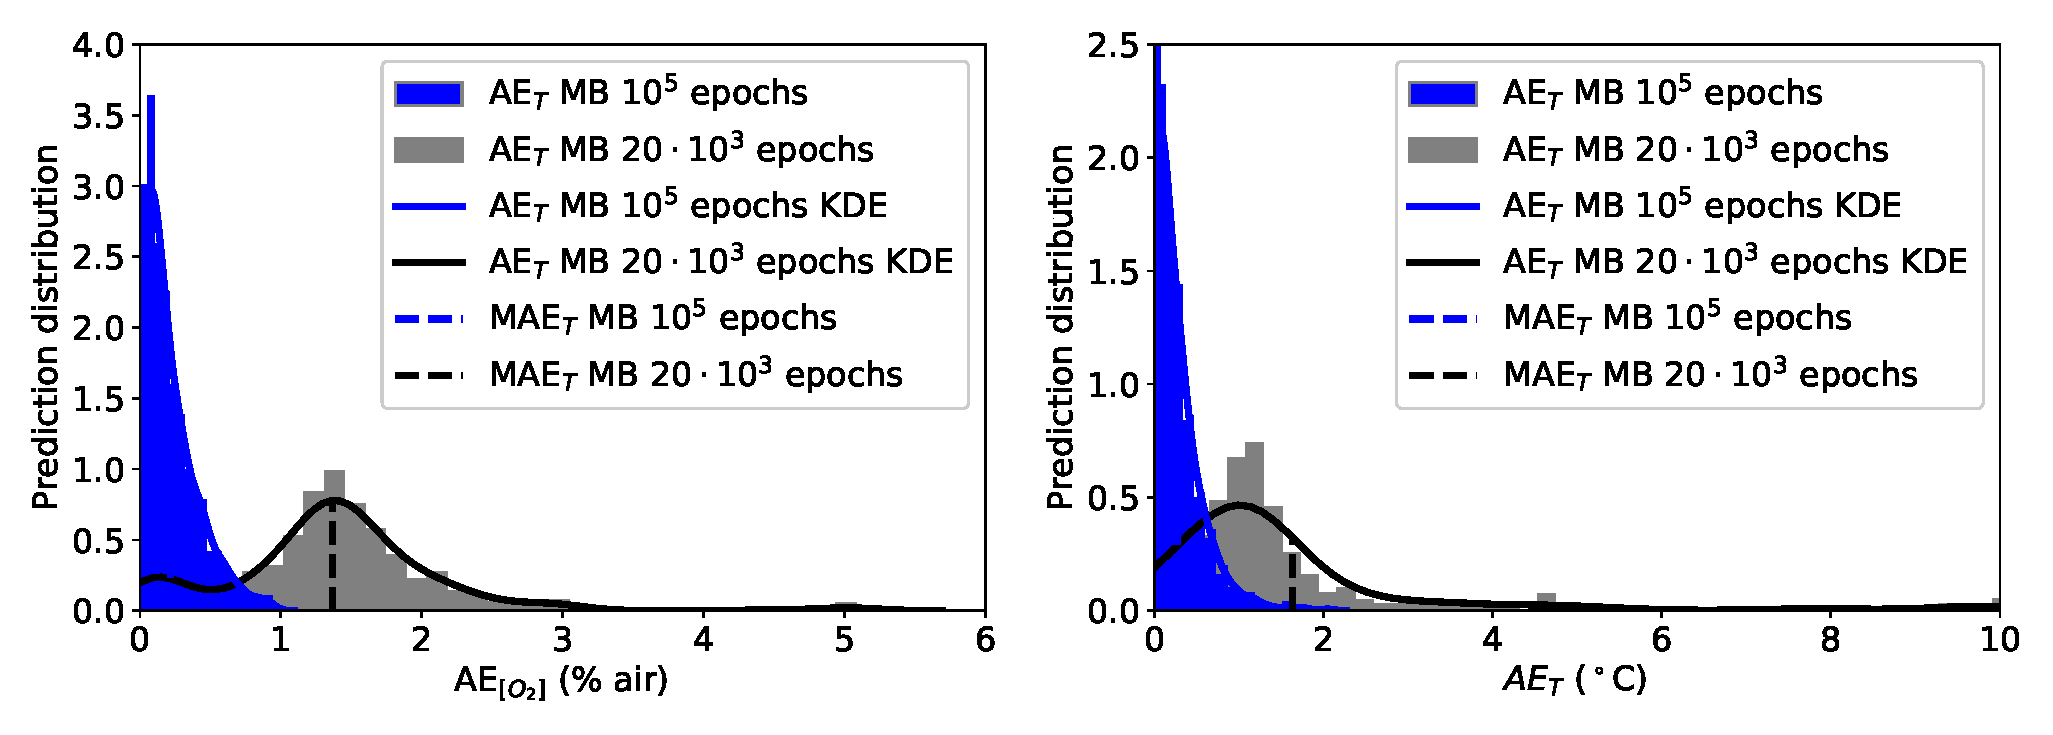
\includegraphics[width=17 cm]{comparison_theta90_20k_vs_100k.eps}
%\caption{Performance of the neural network for the oxygen (left plot) and for the temperature (right plot) predictions: Normalized prediction distribution histogram (columns) and kernel density estimate (KDE) of the distribution of the $AE$s (solid line) using plain gradient descent (GD) and using mini-batches (MB) with a batch size of 32. The corresponding $MAE$ is also shown as a dashed line in each diagram.}
%\label{fig:prediction_distribution_epochs_90}
%\end{figure*}

TIn Figure \ref{fig:KDE_results_all}(E) and \ref{fig:KDE_results_all}(F) predictions distributions are shown when using as input $\theta/\theta_0$, with a mini-batch size of 32 and 20000 epochs. The results are clearly better, especially for the temperature predictions. Training the network with these inputs require roughly 1 hour. Additionally all the predictions for $[O_2]$ lies below 0.87 \% air, and for $T$ lies below 1.7 $^\circ$ C. Additionally training the network in this fashion requires roughly 1 hour. 

%\begin{figure*}[htbp]
%\centering
%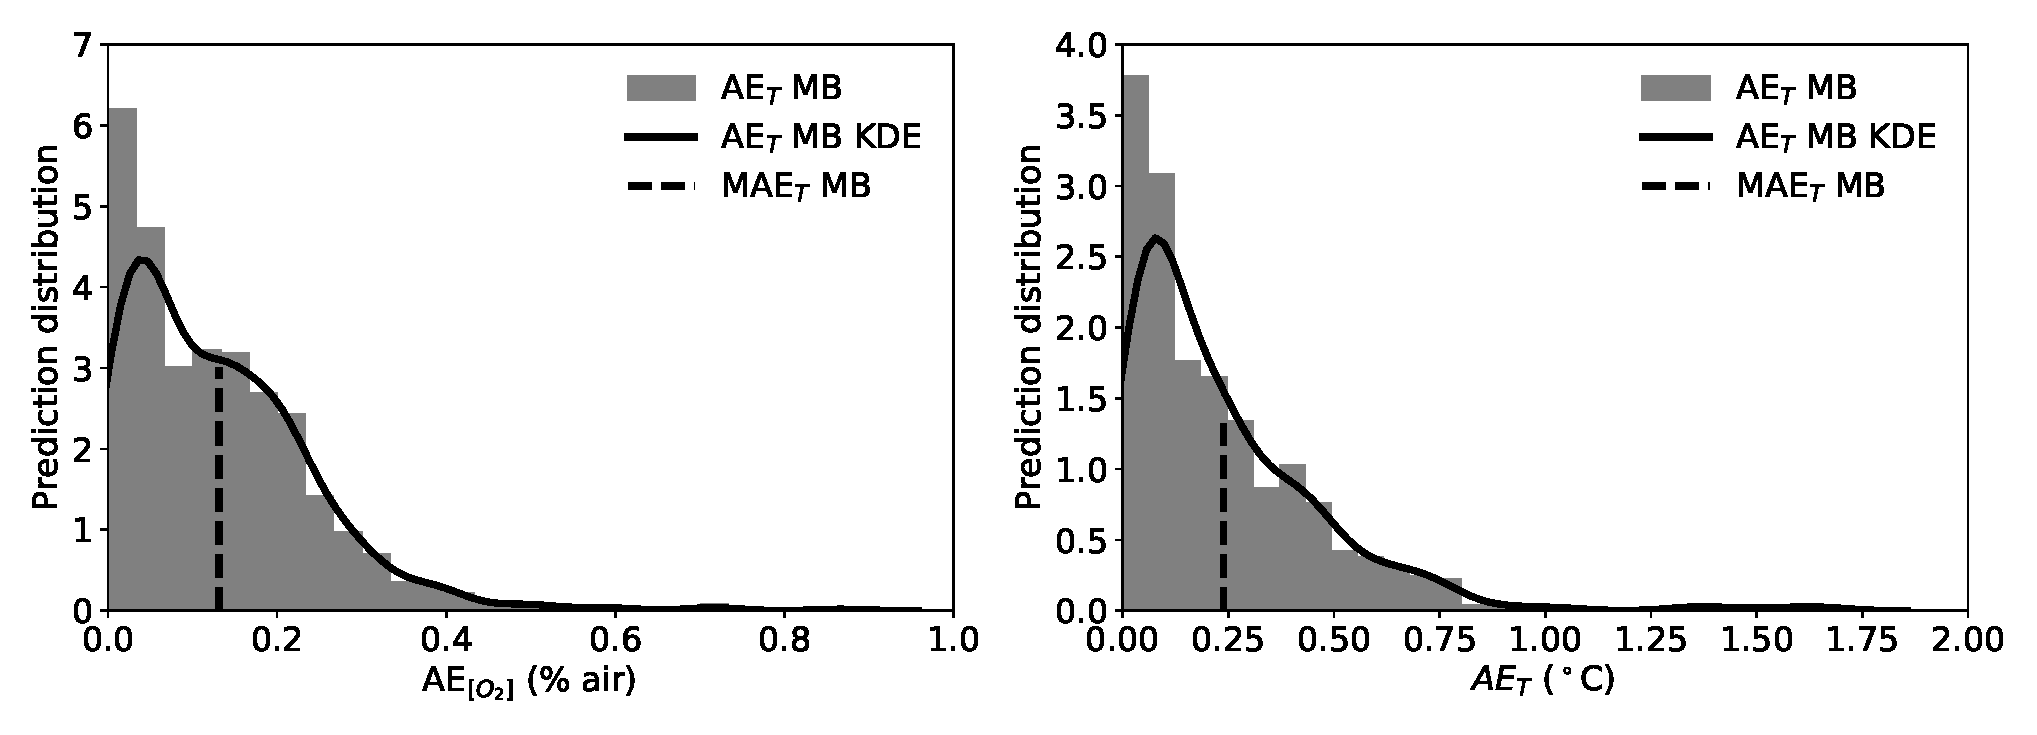
\includegraphics[width=17 cm]{theta_theta0_mb_20k.eps}
%\caption{Performance of the neural network for the oxygen (left plot) and for the temperature (right plot) predictions: Normalized prediction distribution histogram (columns) and kernel density estimate (KDE) of the distribution of the $AE$s (solid line) using plain gradient descent (GD) and using mini-batches (MB) with a batch size of 32. The corresponding $MAE$ is also shown as a dashed line in each diagram.}
%\label{fig:prediction_distribution_theta0}
%\end{figure*}



The performance of the different neural networks is summarized in Table \ref{TableMAE_summary}. 
\begin{table}[hbt]
\centering
\caption {\bf Summary of the performance for the three types of neural network models}

\begin{tabular}{ rccc}
\smallskip 
 Input & Epochs / Batch size & $MAE_{[O_2]}$ & $MAE_{[T]}$  \\ 
 \hline
$\theta / 90^\circ$ & 20'000 / 4000 & 2.38 \% air & 3.63 $^\circ C$\\ 
$\theta / 90^\circ$ & 20'000 / 32 & 1.36\% air & 1.63 $^\circ C$\\ 
$\theta / 90^\circ$& 100'000 / 32 & 0.22 \% air & 0.27 $^\circ C$\\ 
$\theta /\theta_0$ & 20'000 / 32 & 0.13 \% air & 0.24 $^\circ C$\\ 

\end{tabular}
\label{TableMAE_summary}
\end{table}

\subsection{Error Limited Accuracy Plots}

The discussion in the previous sections helps in measuring how the network behave and how good the predictions are, but makes understanding what sensor we could build with such model almost impossible. For a sensors one has to be able to estimate the maximum error for the measurements. To achieve this we developed a completely new metric: the ELA ($\eta$), as defined in section \ref{sektion:ela}, that will allow us to characterise the sensor with a maximum error. As explained previously, $\eta$ is defined only when one chooses a metric $m$. In this section the metric chosen is $m=AE_{[O_2]}$.  

In Figure \ref{fig:ELA_result_comparison} you can see a comparison of $\eta$ versus $\hat m$ for network trained with mini-batches of size 32 and for 20000 and 100000 epochs. The black line are the results for the network that have been trained with $\theta/\theta_0$ as input for 20000 epochs, while the red one with $\theta/90$ as input for 100000 epochs.  
To explain how to read such plot let's consider the two extreme cases. 
\begin{itemize}
\item {\bf Small values of $\hat m$}: $\eta$ will tell us how many predictions lie close to the expected value within the given value of $\hat m$. The smaller $\hat m$ is, the less network predictions will lie within $\pm \hat m$ from the expected values. Therefore the smaller $\hat m$ is, the smaller $\eta$ is. This is clearly reflected in the plot, that for small values of $\hat m$, presents small values of $\eta(\hat m)$.
\item {\bf Bigger values of $\hat m$}: The bigger $\hat m$ is, the more network predictions will lie within $\pm \hat m$ from the expected values. After a certain value of $\hat m$ all the predictions will lie within $\pm \hat m$ from the expected values, effectively giving $\eta = 1$, as reflected on the right side of the plot. 
\end{itemize}

The dashed lines indicates the values of the $AE_{[O_2]}$ for which the predictions would give a 100 accuracy within that error. For example for the network trained with $\theta/90$ as input, if an error of 0.95 \% air is considered acceptable, then the model would predict all the oxygen concentrations within the given error. For the network trained with $\theta/\theta_0$ this value would be 0.87 \% air. 

\begin{figure}[htbp]
\centering
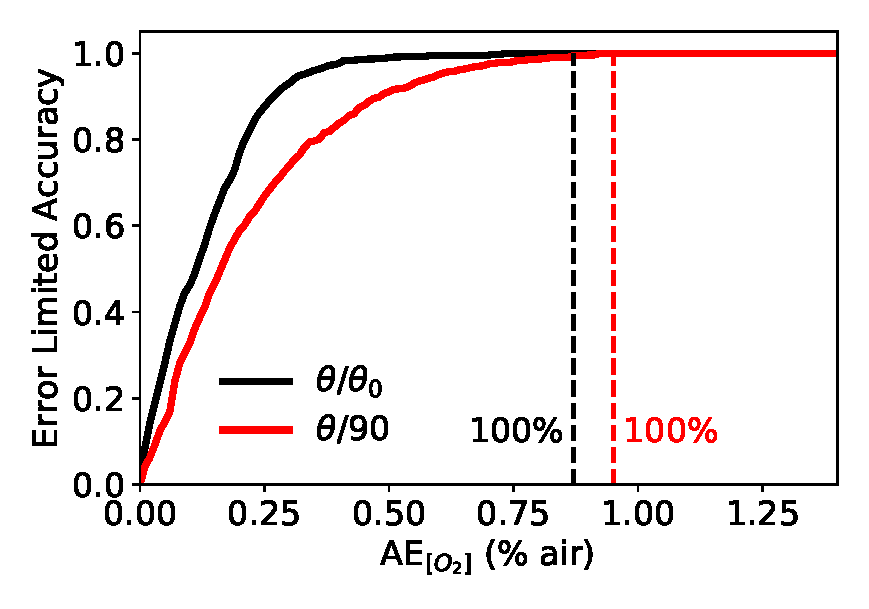
\includegraphics[width=7 cm]{ELA_comparison.eps}
\caption{Comparison of $\eta$ versus $AE_{[O_2]}$ for network trained with mini-batchs of size 32 and for 20000 and 100000 epochs. The black line are the results for the network that have been trained with $\theta/\theta_0$ as input for 20000 epochs, while the red one with $\theta/90$ as input for 100000 epochs. The dashed lines indicates the values of the $AE_{[O_2]}$ for which the predictions would give a 100 accuracy within that error.}
\label{fig:ELA_result_comparison}
\end{figure}


%\begin{figure}[htbp]
%\centering
%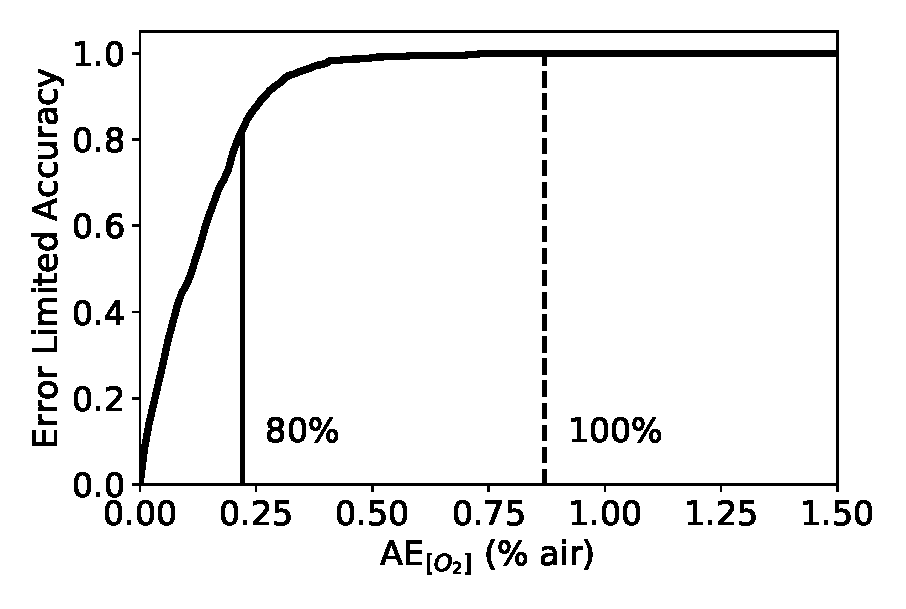
\includegraphics[width=7 cm]{ELA_model_20001_32_1e-3_3x50_2x5_2x5_theta_theta0.eps}
%\caption{ELA...}
%\label{fig:ELA_result_theta0}
%\end{figure}
%
%
%
%\begin{figure}[htbp]
%\centering
%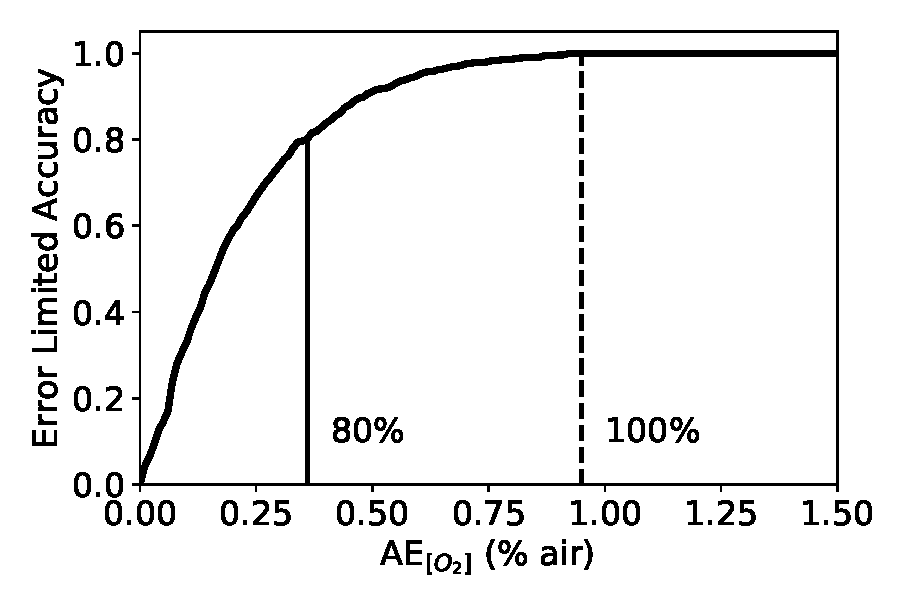
\includegraphics[width=7 cm]{ELA_model_100001_32_1e-3_3x50_2x5_2x5_theta90.eps}
%\caption{ELA...}
%\label{fig:result_theta0}
%\end{figure}


%
%plot theta/theta0 vs frequency for different T (O2 fix) and for different O2 (T fix)
%plot distribution of total AE
%
%temperature can be presicted less well because phase shift depends less from T than from O2
%
%Stability results
%
%temperature cannot be predicted well without dividing for theta 0




\section{Conclusions}

The results in the prediction of the oxygen concentration and temperature show unprecedented accuracy for both parameters, demonstrating that this approach will make a new generation of sensors possible for dual or even multiple sensing. The unprecedented accuracy in predicting both $AE_{[O_2]}$ and $T$ at the same time, from the same set of data, will allow sensors to become easier to build, since no separate temperature measurements are necessary anymore. To be able to estimate what kind of sensor one could build with a given NNM, in this paper a new metric, the ELA ($\eta(\hat m)$), have been proposed to be able to estimate how many predictions like within a certain value of the chosen metric from the expected values.


%\section*{Funding Information}
%National Science Foundation (NSF) (1263236, 0968895, 1102301); The 863 Program (2013AA014402).

%\section*{Acknowledgments}


\section*{Disclosures}

\medskip

\noindent\textbf{Disclosures.} The authors declare no conflicts of interest.


% Bibliography
\bibliography{bibliography}

% Full bibliography will be added automatically on a new page for Optics Letters submissions. This command is ignored for journal article submissions.
% Note that this extra page will not count against page length.
\bibliographyfullrefs{bibliography}

%\printbibliography

%Manual citation list
%\begin{thebibliography}{1}
%\bibitem{Michelucci2017}
%Michelucci, U.
%{\sl Applied Deep Learning - A Case-Based Approach to Understanding Deep Neural Networks}; Apress Media, LLC: New York, NY, USA, 2018; pp. 374--375.

%\bibitem{Kingma2014}
%Kingma, D.P.; Ba, J.
%Adam: A method for stochastic optimization. In Proceedings of 3rd International Conference on Learning Representations, ICLR 2015, San Diego, CA, USA, May 7-9, 2015, pp. 1--15.

%\bibitem{Michelucci2019}
%Michelucci, U.; Baumgartner, M.; Venturini, F.
%Optical oxygen sensing with artificial intelligence.
%{\sl Sensors} {\bf 2019}, {\sl 19}, 777.

˜
%\bibitem{Zhang:14}
%Y.~Zhang, S.~Qiao, L.~Sun, Q.~W. Shi, W.~Huang, %L.~Li, and Z.~Yang,
 % \enquote{Photoinduced active terahertz metamaterials with nanostructured
  %vanadium dioxide film deposited by sol-gel method,} Opt. Express \textbf{22},
  %11070--11078 (2014).
%\end{thebibliography}

\end{document} 